\appendix
\addcontentsline{toc}{chapter}{Appendix} % adds an entry to the table of contents

\chapter{Data collection}

\section{Cantonal data sources}

\subsection*{Parcel boudaries}
\label{app:canton_parcels}

 [ADD FIGURE ON THE AVAILABILITY OF THE DATA]
 
  [ADD TABLE ON THE SOURCES OF THE DATA]

\section{Data pre-processing}

\subsection*{Missing data in the RBD}
\label{app:rbd}
[DEMAND MAPPING LATEX DOCUMENT CONTAINS SOME INFORMATION]

\subsection*{Sub-sectors of industrial and service sectors}
\label{app:noga}

To link the STATENT data (Section \ref{data_rbd_statent}) to different economic activities and to estimate their heat and electricity demand, we use a grouping of NOGA codes into sub-sectors of service and industrial sector based on the mapping suggested in the analysis of the energy use in the industry and services sectors (2019) \cite{bfe_energieverbrauch_2019}, as shown in Table~\ref{tab:noga}. Some NOGA codes are not assigned to any sector, as these codes are considered to have no or a negligible demand for energy and are hence not relevant for the estimation of energy demand (Section \ref{demand_chapter}).

\begin{table}[ht]
\centering
\footnotesize
\caption{Mapping of NOGA codes to sub-sectors of the industry and service sectors}
\label{tab:noga}

\resizebox{\textwidth}{!}{%
\begin{tabular}{llll}
\hline
\textbf{Sector}            & \textbf{Sub-sector}        & \textbf{Sector ID \cite{bfe_energieverbrauch_2019}} & \textbf{NOGA-Code}                                   \\ \hline
\multirow{12}{*}{Industry} & Food production            & 1                            & 10-12                                                \\
                           & Textile / Leather          & 2                            & 13-15                                                \\
                           & Paper / Print              & 3                            & 17, 18                                               \\
                           & Chemistry / Pharmaceutical & 4                            & 20, 21                                               \\
                           & Cement / Concrete          & 5                            & -                                                    \\
                           & Other non-ferrous minerals & 6                            & 23                                                   \\
                           & Metal / Iron               & 7                            & 24                                                   \\
                           & Non-ferrous metals         & 8                            & -                                                    \\
                           & Metal / Tools              & 9                            & 25,27                                                \\
                           & Machines                   & 10                           & 28                                                   \\
                           & Other industries           & 11                           & 7-9, 16, 22, 29-32                                   \\
                           & Construction               & 12                           & 41-43                                                \\ \hline
\multirow{7}{*}{Services}  & Trade                      & 13                           & 45-47, 95                                            \\
                           & Hospitality                & 14                           & 55, 56                                               \\
                           & Credit / Assurances        & 15                           & 64-66                                                \\
                           & Administration             & 16                           & 84                                                   \\
                           & Schools                    & 17                           & 85                                                   \\
                           & Health / Welfare           & 18                           & 75, 86-88                                            \\
                           & Other services             & 19                           & 33, 36-39, 49-53, 58-63, 68-74, 77-82, 85, 90-94, 96 \\ \hline
\end{tabular}%
}
\end{table}

\subsection*{Roads and railways}
\label{app:roads}

To convert roads and railways of the TLM into vector polygons, they are buffered by their width. While road widths are defined for some roads, it has to be derived for several other road objects. We use high-resolution overhead imagery for Switzerland in combination with the TLM and geospatial tools to identify street patterns and measure the typical width for different road and railways types. The resulting mapping between road and railway objects and their width is shown in Table~\ref{tab:roads}.  

\begin{table}[ht]
\centering
\footnotesize
\caption{Mapping of road and railway widths to road types provided in the TLM.}
\label{tab:roads}

\begin{tabular}{llll}
\hline
\textbf{Type}            & \textbf{Description}    & \textbf{Object ID(s) \cite{swisstopo_swisstlm3d_2018}} & \textbf{Width (m)} \\ \hline
\multirow{5}{*}{Road}    & Driveways           & 0, 1, 5, 6                      & 6                  \\
                         & Connecting roads    & 4                               & 6                  \\
                         & Road (3,4,6,8,10 m) & 8-11, 20                        & 3-10*              \\
                         & Regional road       & 21                              & 15                 \\
                         & Highway             & 2                               & 30                 \\ \hline
\multirow{3}{*}{Railway} & Normal track        & 0                               & 5                  \\
                         & Narrow track        & 2, 4                            & 3                  \\
                         & Small train         & 5                               & 3                  \\ \hline
\multicolumn{4}{l}{* Road width given as line attribute}                                             
\end{tabular}
\end{table}


\chapter{Solar PV potential estimation}

\section{Tuning of Machine Learning models}
\label{app:tuning}
%
For the tuning of the ML models (see Section~\ref{methods_ML} for details), the mean-squared error (MSE) is used as means to assess performance and is evaluated on a validation set, which is randomly sampled as 20\% of the training data. A k-fold cross-validation procedure, as suggested in \cite{leuenberger_extreme_2015}, is not applied here as it is beneficial for relatively small data sizes but does not bring significant improvements for large datasets as used here \cite{heskes_practical_1997}.

This section borrows from \citet{walch_spatio-temporal_2019} to provide a more complete overview of the tuning procedure for Extreme Learning Machine Ensembles in the context of the estimation of global solar radiation.

\subsection*{Extreme Learning Machine Ensemble}
\label{app:tune_ELM}

To estimate $G_h$ and $G_B$ (Section~\ref{irrad}), we use training data from 11,243 pixel coordinates in Switzerland and for 4,663 hours with non-zero solar radiation, which are split into 12 monthly subsets (see Section~\ref{data_solarRad}).
The training data for $\rho$ are 365 daily values for each coordinate. 
The output grid of $200 \times 200$ m$^2$ pixels results in a prediction set of 1.04 M locations, with 146 non-zero MMH time steps (for $G_h, G_B$) or 12 monthly values (for $\rho$).  For model training, each variable is normalized to zero mean and unit variance.
%
As Extreme Learning Machines (ELM) are single-layer neural networks, the ELM-E has two hyper-parameters that are tuned, (i) the number of nodes of the hidden layer of each neural network $m$, and (ii) the number of ELM in the ensemble $n$. While the number of nodes significantly impacts the generalization performance of the algorithm, an increased ensemble size improves the stability of the algorithm and hence $n$ is mainly limited by computational time. % MAKE SURE THESE AGREE WITH ML SECTION

\begin{figure}[tb]
\centering
\begin{subfigure}{.49\textwidth}
  \centering
  % include second image
  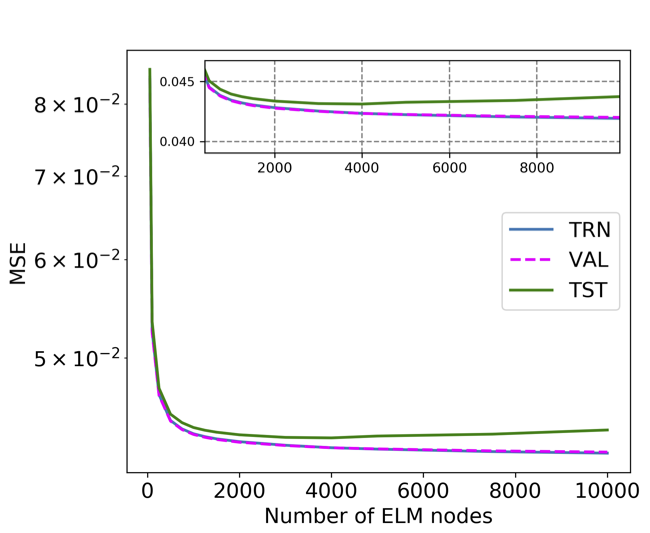
\includegraphics[width=\linewidth]{Figs/ELM_error.png}  
  \caption{}
  \label{figa:ELM_training}
\end{subfigure}
\begin{subfigure}{.49\textwidth}
  \centering
  % include first image
  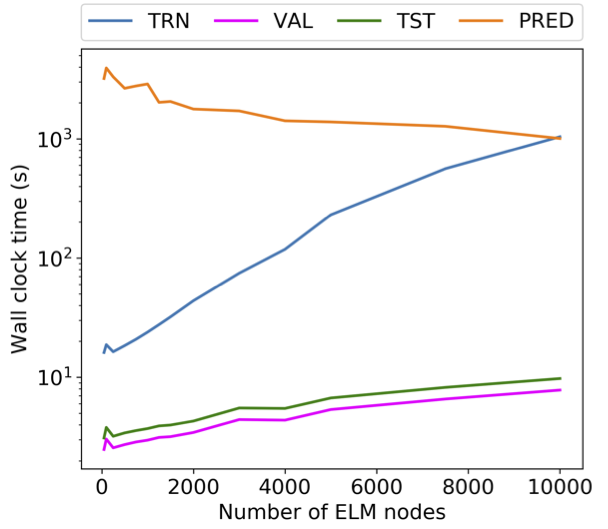
\includegraphics[width=\linewidth]{Figs/ELM_time.png}  
  \caption{}
  \label{figb:ELM_training}
\end{subfigure}
\caption{ELM tuning, including (a) wall clock time per model and (b) training (TRN), validation (VAL) and test (TST) MSE, both as a function of number of nodes.}
\label{fig:ELM_training}
\end{figure}

The tuning of ELM hyper-parameters based on the MSE minimization of the validation data (VAL) is performed by scanning $n$ ranging from 10 to 100 and $m$ from 50 to 10000. Preliminary studies showed that this is a reasonable range, given that higher values come at high computational cost without resulting in significant improvements. Depending on $m$, the wall clock time needed for training a single model can range from few seconds up to 15-20 minutes, as shown in Fig.~\ref{figa:ELM_training}, on a GPU accelerated machine using one K40 NVIDIA card. The optimal number of $n$ and $m$ is hence a trade-off between the computational time required by the model and the exhibited performance on the VAL sample.

The tuning procedure of $G_h$ for the month of June is visualised in Fig.~\ref{figa:ELM_training} and Fig.~\ref{figb:ELM_training}, while a numerical comparison of MSE, training and prediction times is provided in Table~\ref{tab:ELM_tuning}. The computational time (Fig.~\ref{figa:ELM_training}) is dominated by the evaluation of the chosen model on the dense spatial grid used for the GHI predictions (PRED). The MSE for VAL (Fig.~\ref{figb:ELM_training}), representing the model performance, steeply falls before 500 nodes and then stabilizes on low values without significant improvement when further increasing $m$, suggesting a minimum model size of $m = 500$. While the given data is for $G_h$ in June, similar trends exist for the other months, for $G_B$ and $\rho$. 
Considering also the computational time, which constantly increases with $m$, we choose the model hyper-parameters as a trade-off between performance and computational efficiency. 
The selected hyper-parameters are $m=1000, n=50$ for $G_h$ and $G_B$ and $m=1000, n=30$ for $\rho$.
The model performance on the test set (TST) shows a-posteriori that this choice is appropriate.

\begin{table}[tb]
\centering
\footnotesize
\caption{Results of the tuning of $m$, showing the trade-off between the validation MSE and training and prediction times (per ELM), for $G_h$ in June. The selected value for $m$ is shown in bold.}
\label{tab:ELM_tuning}

    \begin{tabular}{lccccccc}
    \hline
    \textit{m}          & 50    & 100   & 500   & \textbf{1000}  & 2000  & 5000  & 10000 \\ \hline
    Validation MSE      & 0.084 & 0.052 & 0.044 & \textbf{0.043} & 0.043 & 0.042 & 0.042 \\
    Training time (s)   & 16    & 18    & 18    & \textbf{23}    & 43    & 230   & 1040  \\
    Prediction time (s) & 2.5   & 3.0   & 2.7   & \textbf{3.0}   & 3.4   & 5.4   & 7.8   \\ \hline
    \end{tabular}
\end{table}

\subsection*{Random Forest}
\label{app:tune_RF}

Random Forests are used for two separate models, to estimate $C_{\mathit{pv}}$ (Section~\ref{panels}) and $C_{sh}$ (Section~\ref{shade}). Due to the smaller size of the data as compared to the ELM-E, a 5-fold cross-validation is applied. It splits the data into 5 subsets, from which 5 separate models are trained and validated each on a different subset. 
The RF has three main hyper-parameters which can be tuned: the number of trees in the ensemble ($n$), the minimum number of samples in each leaf node ($l$), and the number of features ($m$) which are randomly considered for splitting at each node. $m$ determines the level of randomization within each decision tree, $l$ impacts the level of smoothing of the predictions, while $n$ improves the robustness of the model, and is primarily limited by computational time \cite{breiman_random_2001}.
The selected hyper-parameters for both models are  $l = 3$, $m = 5$ and $n = 1000$. It should be noted that the RF is much less prone to small deviations in the model hyper-parameters than the ELM-E.

%%%%%%%%%%%%%%%%%%%%%%%%%%%%%%%%%%%%%%%%%%%%%%%%%%%%%%%

\section{Geospatial algorithms}

\subsection*{Virtual installation of PV panels}
\label{app:virtualPV}

Algorithm~\ref{alg:panels} details the geospatial algorithm that is implemented to virtually install PV panels on roof surfaces. It uses the python \texttt{geopandas} library \cite{kelsey_jordahl_geopandas/geopandas:_2019}. 
The output of the geospatial algorithm, $C_{\mathit{pv}}$, is calculated for each roof surface as the ratio between the roof area covered by $N_{\mathit{panels}}$ virtual panels, each of area $A_{\mathit{panel}}$, and the tilted area $A_{t}$ of the roof surfaces: 

\begin{equation}
\label{eq:cpv}
C_{\mathit{pv}} = \frac{N_{\mathit{panels}} \times A_{\mathit{panel}}}{A_t}
\end{equation}

\begin{algorithm}[htbp]
\caption{PV panel placement on rooftop polygons}
\label{alg:panels}
\begin{algorithmic}[1]
  \footnotesize
  \State Rotate roof surfaces to face south
  \State Create inside buffers (0.4m) along the roof edges
  \State Project PV panel dimensions for each tilted roof
  \Statex \textbf{for all} roof surfaces:
    \State \qquad Place rectangular grid on south-facing roof
    \State \qquad Remove grid cells (panels) outside roof surface
    \State \qquad Count panels and rotate to roof aspect
  \State Compute panelled area and panelled area ratio
\end{algorithmic}
\end{algorithm}

\subsection*{Shading effects}
\label{app:shade}

The shading effects, namely $S_{sh}$ and $C_{sh}$, are computed using horizon maps for each azimuth angle of the sun. Algorithm~\ref{alg:shade} describes the steps to extract $S_{sh}$ and $C_{sh}$ from the horizon maps.
The computation of these maps is the most computationally expensive step in the estimation of hourly RPV potential. Hence, several measures are taken to assure the feasibility of the approach:

\begin{enumerate}
    \item Horizon maps are computed in bins of $5^\circ$ for south-east to south-west sun azimuths (110-250$^\circ$), and in bins of $10^\circ$ for east (60-110$^\circ$) and west (250-300$^\circ$) azimuths, where solar radiation is low. Thus, only 38 maps need to be computed.
    \item The horizon distance is 100 m, i.e. a radius of 100 m is considered around each pixel to compute horizons. In Switzerland, where few high-rise buildings exist, this threshold is suitable to estimate the shading effects from surrounding trees and buildings.
    \item The algorithm is implemented using the GRASS GIS engine~\cite{neteler_grass_2012}. The Swiss terrain is split into 16 sub-regions and processed in parallel to reduce the computational time from $\sim$1000 to $\sim$30 hours. 
    
\end{enumerate}

\begin{algorithm}[htbp]
\caption{Computation of shading effects on rooftops}
\label{alg:shade}
\begin{algorithmic}[1]
  \footnotesize
  \State Compute horizon maps from DSM for 38 angle bins
  \State Crop horizon maps over (rasterized) roofs
  \Statex \textbf{for all} $t$:
    \State \qquad Apply binary filter to horizon maps using the solar position
  \State Average binary shading masks over \textit{t} (sun exposure map)
  \State Extract roof areas with sun exposure $< 40\%$
  \State Compute \textit{shaded area coefficient} $C_{sh}$
  \Statex \textbf{for all} $t$:
  	\State \qquad Extract roof areas with sun exposure $> 40\%$
    \State \qquad Compute \textit{hourly shading fraction} $S_{sh}(t)$
\end{algorithmic}
\end{algorithm}

\subsection*{Sky view factor}

The sky view factor is computed from similar horizon maps as described above for 32 equally spaced azimuth bins and a horizon distance of 100 m, using the \textit{skyview} add-on for GRASS GIS~\cite{zaksek_sky-view_2011}. The computation is performed in parallel over 64 sub-regions.



\section{Configuration of solar panels on flat roofs}
\label{app_flat}

\begin{figure}[tb]
	\centering
	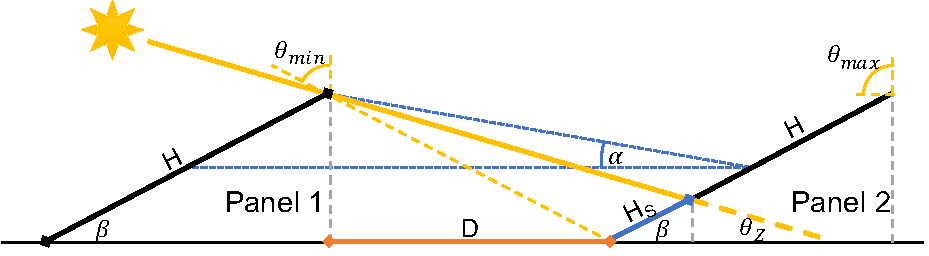
\includegraphics[width=.7\linewidth]{Figs/flat_panels2.pdf}  
	\caption{Geometric model for calculating mutual shading between panel rows, simplified in 2 dimensions and assuming infinite length of the panel rows.}
	\label{fig:flat_concept}
\end{figure}

In this work, panels on flat roofs are not modelled as flat panels on the surface, but instead they are modelled as rows of south-facing panels. For this, the tilt angle ($\beta$) and the distance between adjacent rows of panels ($D$) have to be chosen. We use a 2-dimensional geometric model, shown in Figure~\ref{fig:flat_concept}, to simulate the PV output of roofs with different panel configurations (i.e. different values for $\beta$ and $D$). The optimal parameters are then selected as a trade-off between the simulated PV output and the economic feasibility (indicated by the capacity factor).

The simulation also accounts for mutual shading between panel rows, which reduces the direct tilted radiation and the skyview factor.
The additional direct shading ($S_{\mathit{flat}}$) of a panel at a time $t$ is given by the ratio of the shaded panel height ($H_s$) to the total panel height ($H$). For computational reasons, we only consider distances which are integer multiples of the projected panel height, i.e. $D=n*H \cos{\beta}$. $S_{\mathit{flat}}(t)$ is hence given by:

\begin{equation}
\label{eq:flat_Sh}
    S_{\mathit{flat}}(t) = \frac{H_s}{H} =  \frac{1 - n \frac{\tan{\theta_Z}}{\tan{\beta}}}
               {1 + \frac{\tan{\theta_Z}}{\tan{\beta}}}
\end{equation}

where $\theta_z$ denotes the zenith angle of the sun. As $S_{sh}$ is bounded in the interval $[0,1]$, the minimum and maximum zenith angles for the mutual shading effects are:

\begin{equation}
\begin{aligned}
\label{eq:flat_theta}
    \theta_{min} & = 90^\circ - \tanh(\tfrac{\tan{\beta}}{n} ) \\
    \theta_{max} & = 90^\circ
\end{aligned}
\end{equation}

In addition to direct shading, the installation of adjacent panel rows reduces the skyview factor ($\mathit{SVF}_{\mathit{flat}}$). The SVF is computed as the fraction of a semisphere placed in the center of the panel that is covered by the previous panel row. In the 2D case, this fraction is represented by the angle $\alpha$ shown in Fig.~\ref{fig:flat_concept}. The $\mathit{SVF}_{\mathit{flat}}$ is hence computed as:

\begin{equation}
\begin{aligned}
\label{eq:flat_svf}
    \mathit{SVF}_{\mathit{flat}} & = \frac{\alpha}{\pi} \\
    \tan{\alpha} & = \frac{\tan{\beta}}{2 n + 1}
\end{aligned}
\end{equation}

To choose the optimal tilt angle and distance between panel rows, we compute the annual PV output per unit area of roof surface ($\mathit{Ssh}_{\mathit{out}}$, in kWh$_{\mathit{pv}}$/m$^2_{\mathit{roof}}$) and the annual capacity factor ($\mathit{CF}$, in kWh$_{\mathit{pv}}$/kWp):

\begin{equation}
\begin{aligned}
\label{eq:flat_pv}
    \mathit{PV}_{\mathit{out}} &= \sum_t G_t(t) * \bar{A}_{\mathit{panels}} * \eta_{PV} \\
    \mathit{CF} &= \frac{A_{\mathit{cap}}}{\bar{A}_{\mathit{panels}}} \mathit{PV}_{\mathit{out}}
\end{aligned}
\end{equation}

where $\bar{A}_{\mathit{panels}}$ denotes the normalized panelled area, i.e. the PV panel area per unit of roof surface (in m$^2_{\mathit{panels}}$/m$^2_{\mathit{roof}}$), and $A_{\mathit{cap}}$ denotes the area required to install a peak power of 1 kWp. $A_{\mathit{cap}}$ is estimated at 6 m$^2$/kWp. $\bar{A}_{\mathit{panels}}$ is given by:
\begin{equation}
\label{eq:flat_n_norm}
    \bar{A}_{\mathit{panels}} = \frac{1}{(n+1) \cos{\beta}}
\end{equation}

\begin{figure}[tb]
	\centering
	\begin{subfigure}{.49\textwidth}
		\centering
		% include second image
		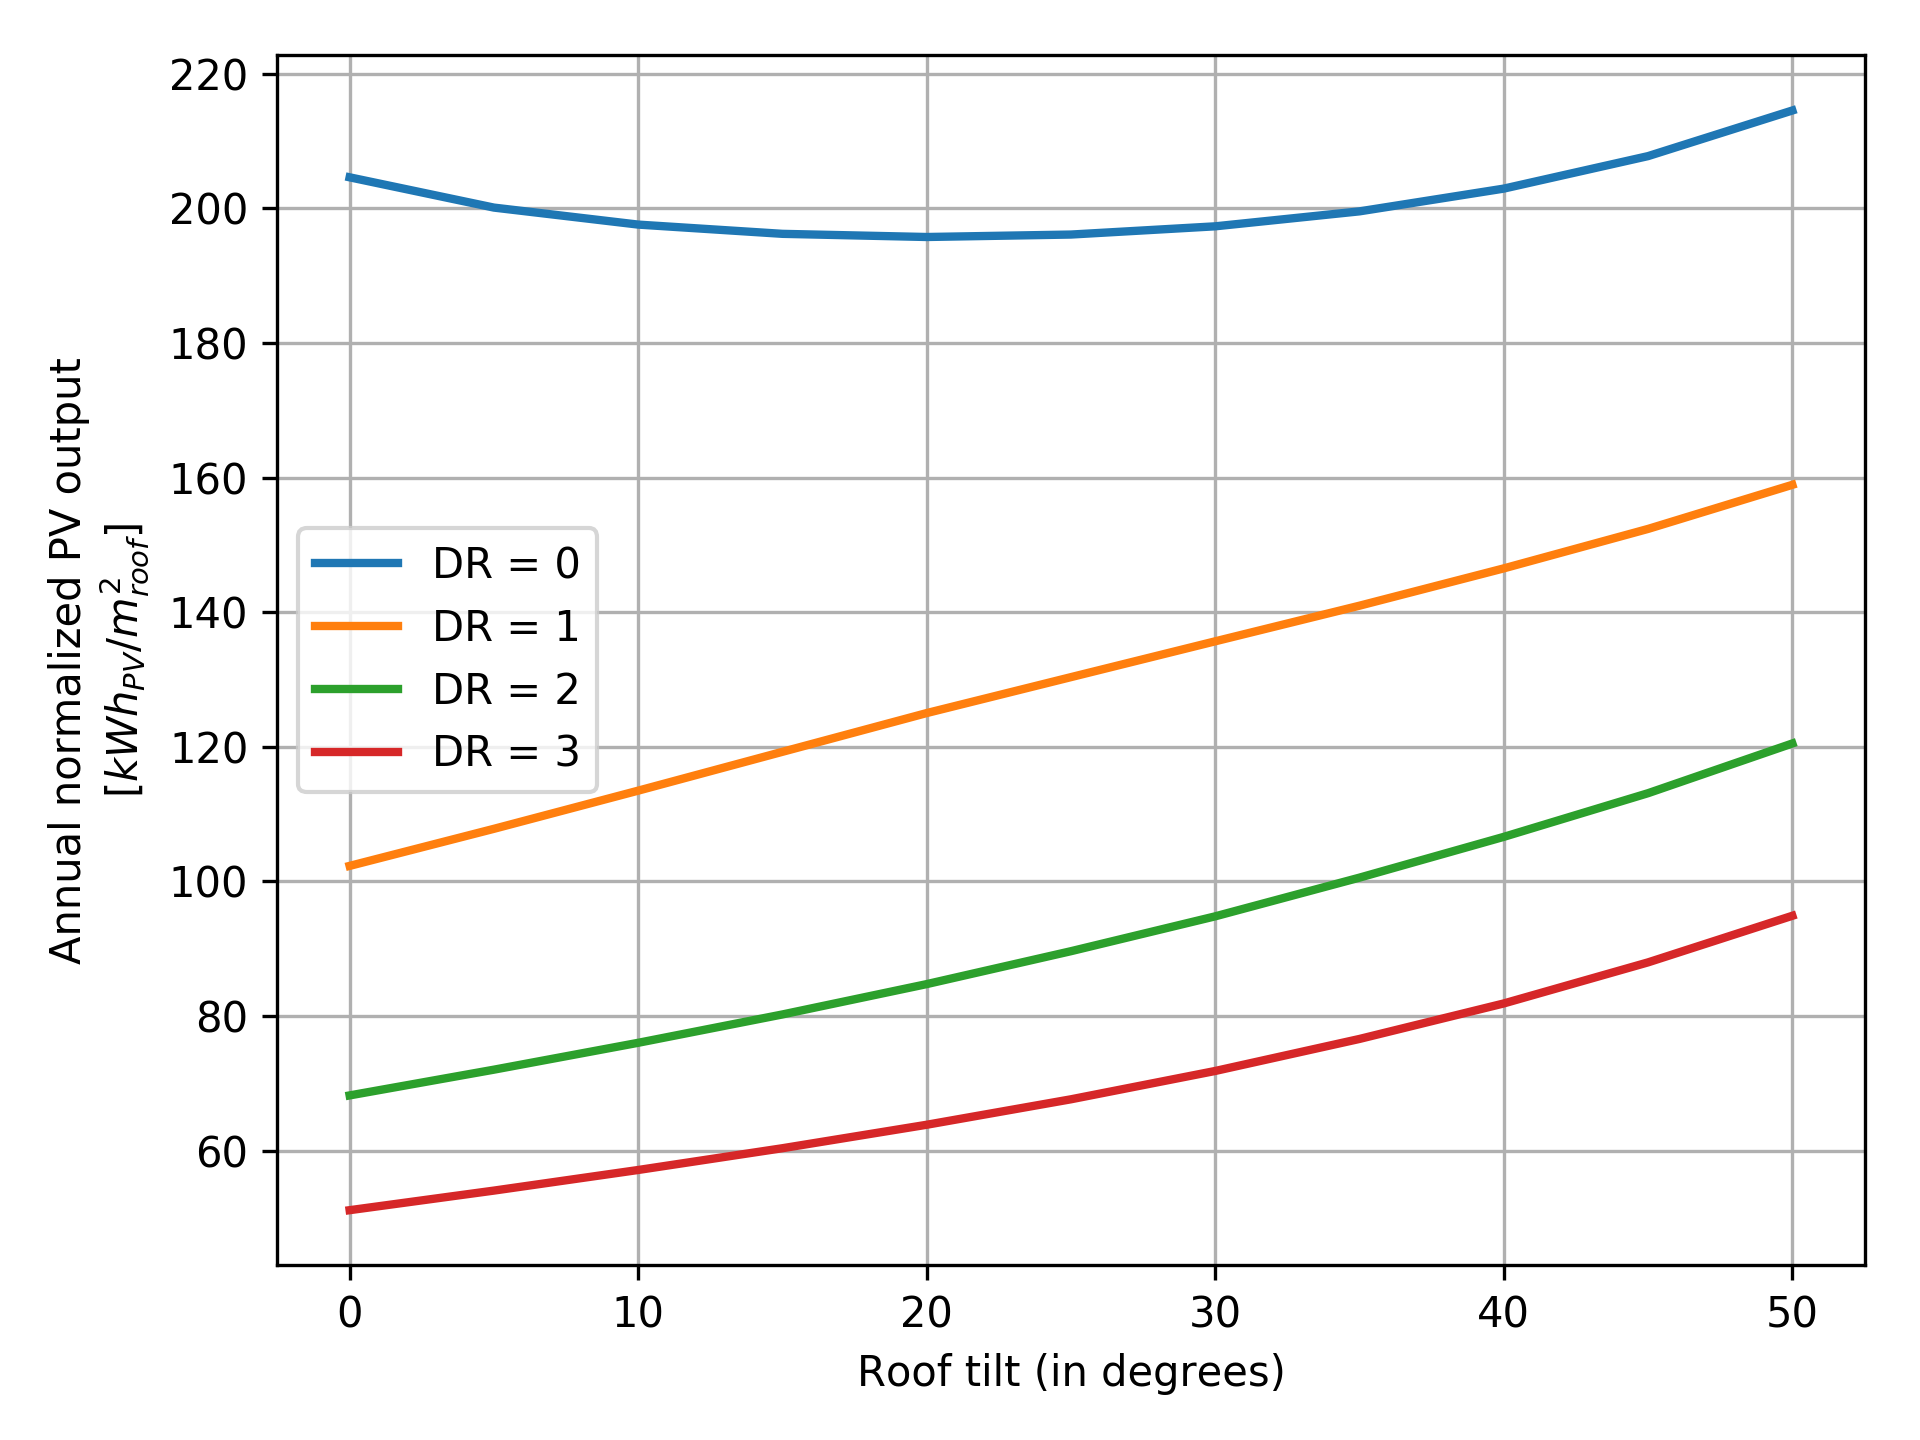
\includegraphics[width=.8\linewidth]{Figs/mututal_pv_out.png}  
	\end{subfigure}
	\begin{subfigure}{.49\textwidth}
		\centering
		% include first image
		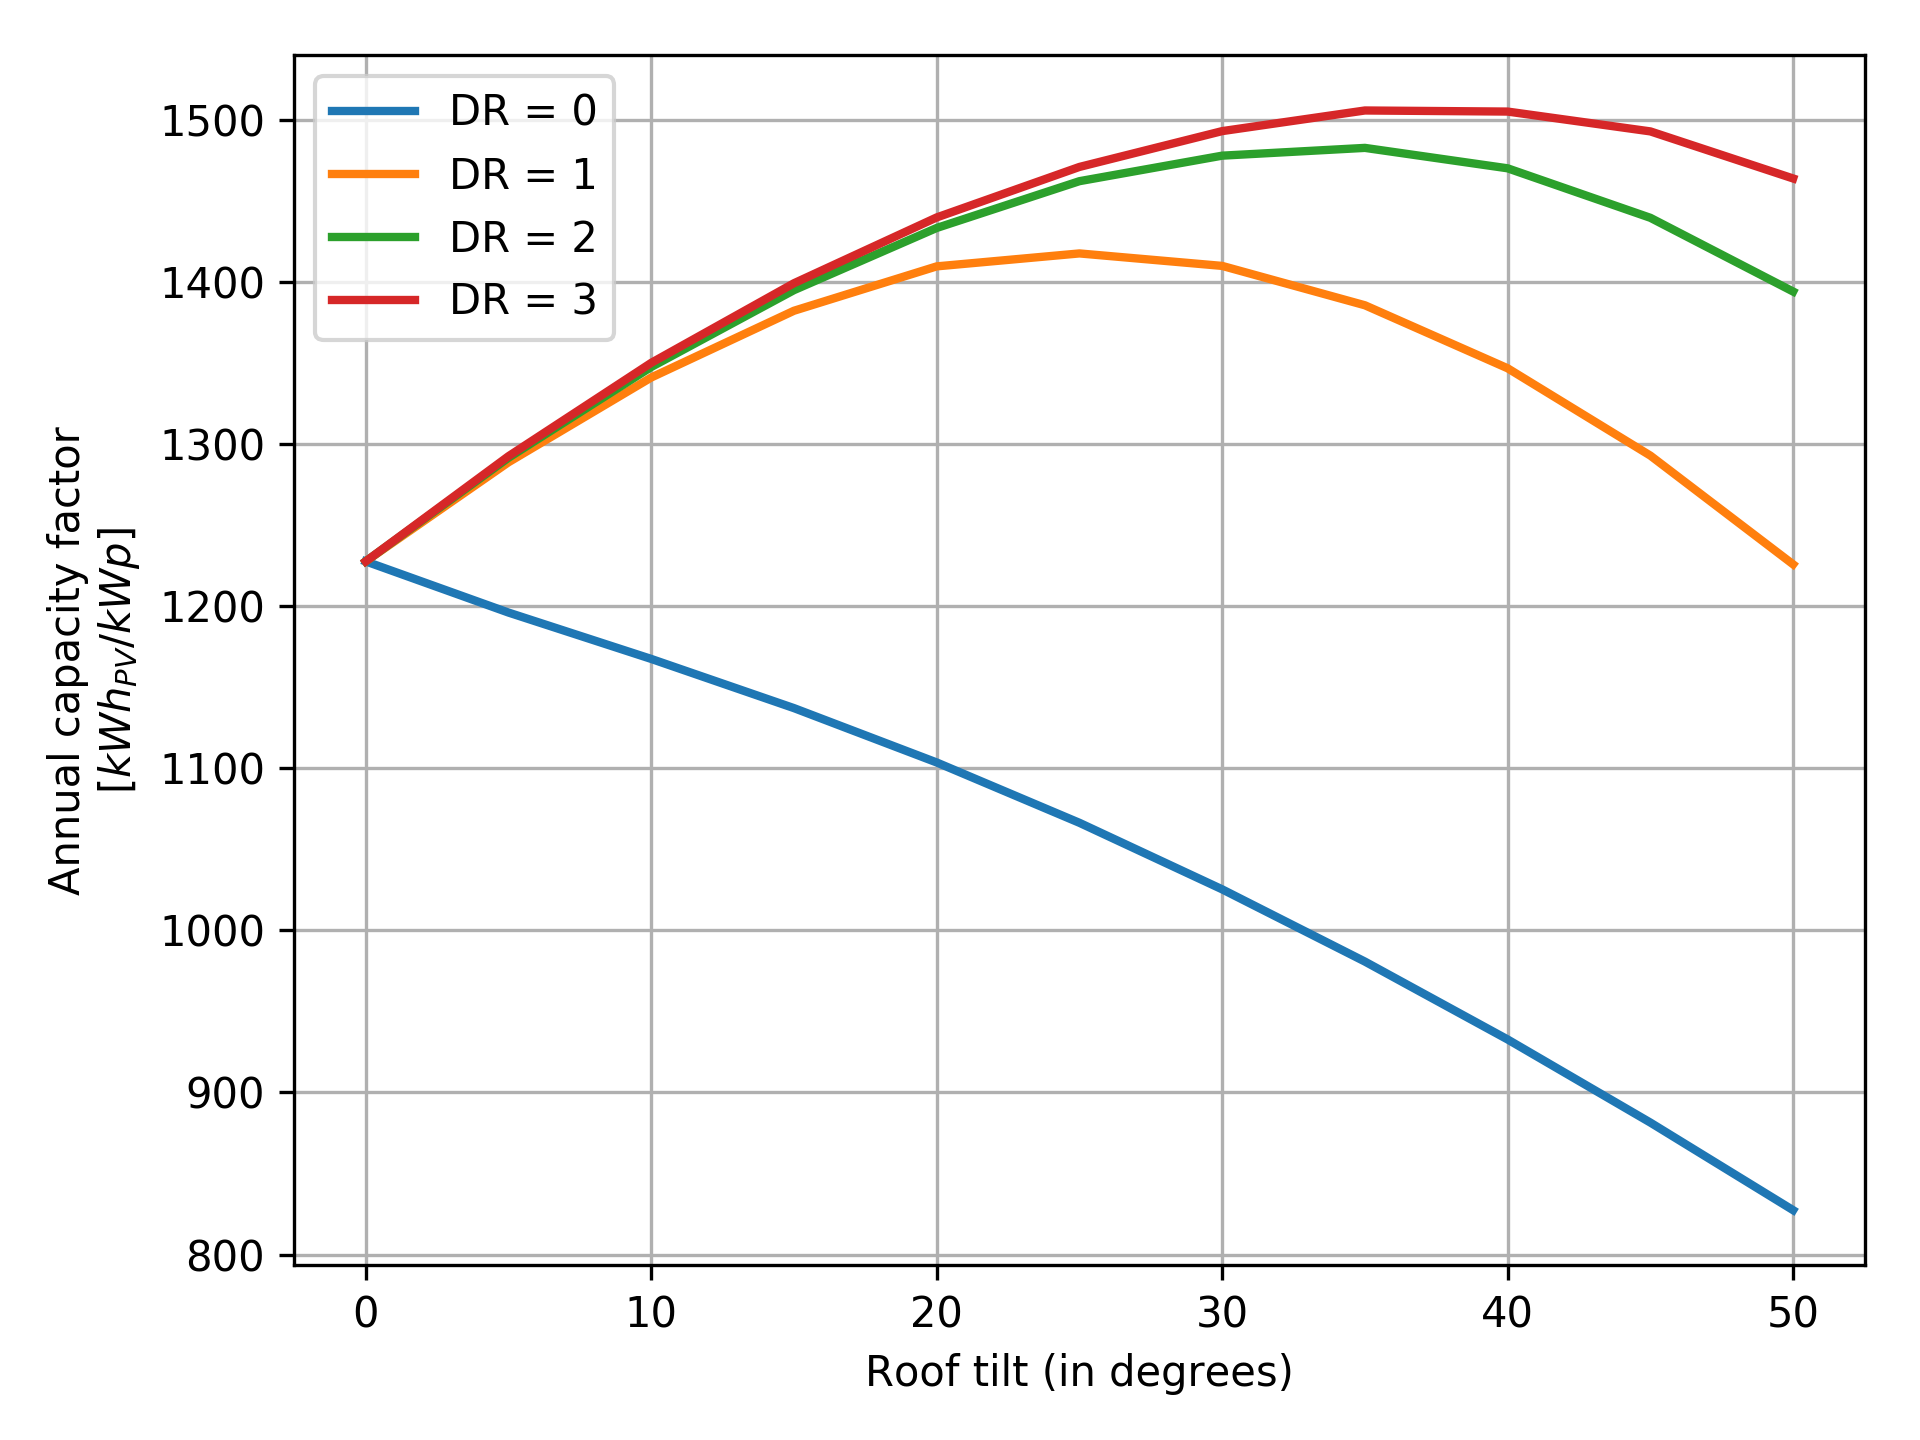
\includegraphics[width=.8\linewidth]{Figs/mututal_cap_factor.png}  
	\end{subfigure}
	\caption{a) PV output per unit of roof area and b) capacity factor, for different configurations of panel tilt and distance between panels on flat rooftops}
	\label{fig:flat_panels}
\end{figure}

The results for simulating $\mathit{PV}_{\mathit{out}}$ and $\mathit{CF}$ for different $\beta$ and $n$ is shown in Figure \ref{fig:flat_panels}.
The simulation assumes a nominal horizontal radiation of 1000 W/m$^2$ and accounts for the effects of mutual shading between rows ($S_{\mathit{flat}}$ and $\mathit{SVF}_{\mathit{flat}}$). 
DR in Fig.~\ref{fig:flat_panels} denotes the "distance ratio", i.e. the integer multiple $n$. While total PV output is largest for rows without spacing, this configuration is the least economically feasible, as it has the lowest $\mathit{CF}$. If panel rows are placed with some spacing, the PV output is higher and the capacity factor peaks at a panel tilt of 25$^\circ$-50$^\circ$. 
Based on these results, we choose a panel tilt of 30$^\circ$ and a distance of 1 panel height ($n=1$) for flat roofs as a trade-off between PV output and capacity factor.


%%%%%%%%%%%%%%%%%%%%%%%%%%%%%%%%%%%%%%%%%%%%%%%%%%%%%%%

\section{Uncertainty propagation for tilted radiation}
\label{unc_Gt}

The variance and covariance of the three addends in Eq.~(\ref{eq:irrad}) (labelled $B, D, R$ in Eq.~(\ref{eq:irrad_unc})) are computed from the mean and variance of the horizontal radiation ($G_{B,D,h}$, $\sigma^2_{GB,GD,Gh}$), the partly shaded factor ($(1-S_{sh})$, $\sigma^2_{sh}$) and the sky view factor ($\mathit{SVF}$, $\sigma^2_{\mathit{SVF}}$) such that:

\begin{equation}
\begin{aligned}
% Definition of variance of beam component
\sigma^2_{B} & = F_{B}^2 (\sigma^2_{\mathit{Ssh}} G_B^2 + \sigma^2_{GB} (1-S_{sh})^2 + \sigma^2_{\mathit{Ssh}} \sigma^2_{GB}) \\
% Definition of variance of diffuse component     
\sigma^2_{D} & = F_{D}^2 (\sigma^2_{\mathit{SVF}} G_D^2 + \sigma^2_{GD} \mathit{SVF}^2 + \sigma^2_{\mathit{SVF}} \sigma^2_{GD}) \\
% Definition of variance of reflected component
\sigma^2_{R}&  = F_{R}^2 \sigma^2_{Gh}
\end{aligned}
\end{equation}

where $F_{B}, F_{D}, F_{R}$ are the beam, diffusion and reflection factors introduced in Eq.~\ref{eq:tilted_irrad_simplified}. 
Under the assumptions in Section~\ref{unc_prop}, we derive the covariances between the beam, diffuse and reflected components of $G_t$ as a function of the covariances between the horizontal radiation components, as well as the covariance between the shading and the SVF, such that:

\begin{equation}
\begin{aligned}
% covariance between direct and diffuse
\mathrm{Cov}(B, D) & = F_{B}  F_{D} \times (\mathrm{Cov}(G_B, G_D) \times \mathrm{Cov}(S_{sh}, \mathit{SVF}) \\
& + G_B  G_D \times \mathrm{Cov}(S_{sh}, \mathit{SVF}) \\
& + (1-S_{sh}) \times \mathit{SVF} \times \mathrm{Cov}(G_B, G_D)) \\
% covariance between direct and reflected
\mathrm{Cov}(B, R) & = F_{B}  F_{R} \times (1-S_{sh}) \times \mathrm{Cov}(G_B, G_h) \\
% covariance between diffuse and reflected
\mathrm{Cov}(D, R) & = F_{D}  F_{R} \times \mathit{SVF}  \times      \mathrm{Cov}(G_D, G_h) 
\end{aligned}
\end{equation}

where the covariances $\mathrm{Cov}(G_h, G_D)$ and $\mathrm{Cov}(G_B, G_D)$ are computed from $\sigma_{Gh}, \sigma_{GB}$ and $\sigma_{GD}$ in analogy to Eq.~(\ref{eq:unc_GD}).

%%%%%%%%%%%%%%%%%%%%%%
%%%%%%%%%%%%%%%%%%%%%%%

\chapter{Geothermal potential estimation}

\section{Analytical models and comparison}
\label{app:allModels}

As explained in Section~\ref{geo_models}, three analytical solutions exist for modelling the thermal dynamics in the ground due to heat extraction from a BHE: the Finite Line Source (FLS), the Infinite Line Source (ILS) and Eskilson's approximation (Esk) \cite{pahud_geothermal_2002}. The transient and steady-state behaviour of the three models is explained below, followed by a comparison in terms of accuracy (with respect to the FLS) and computational time. The comparison is performed based on own simulations using the equations provided below.

\textbf{Finite Line Source (FLS)}. 
The FLS describes the most accurate analytic model used in the literature. It is a solution to the heat conduction equation that satisfies the boundary conditions $T(r, z=0, t=0) = 0$. The g-function of the transient solution is given by \citep{pahud_geothermal_2002}:

\begin{equation}
\label{eq:FLS}
    \mathrm{g}_{FLS}(r, z, t) = \frac{1}{2} \int_{D}^{D+H} \left( \frac{1}{r_+} \mathrm{erfc}\left(\frac{r_+}{\sqrt{4 \alpha t}}\right) - \frac{1}{r_-}\mathrm{erfc}\left(\frac{r_-}{\sqrt{4 \alpha t}}\right) \right) ds
\end{equation}

where
\begin{equation*}
    r_+ = \sqrt{r^2 + (z - s)^2}, \quad r_- = \sqrt{r^2 + (z + s)^2}
\end{equation*}

\begin{equation*}
   \mathrm{erfc}(x) = \frac{2}{\sqrt{\pi}} \int_{x}^{\infty} e^{-\mu^2} d\mu
\end{equation*}

The steady-state solution (valid for $t > t_{ss}$) is defined as:

\begin{equation}
\label{eq:FLS_ss}
    \mathrm{g}_{FLS,ss}(r, z) = \frac{1}{2} \int_{D}^{D+H} \left( \frac{1}{r_+} - \frac{1}{r_-} \right) ds
\end{equation}
For many borehole applications, the mean temperature along the borehole length is of interest. This can be obtained by integrating $\mathrm{g}_{FLS}(r, z, t) $ along the $z$-axis. \citet{claesson_analytical_2011} provide the analytical solution described in Section~\ref{geo_models}.

\begin{comment}

\begin{equation}
\label{eq:FLS_int}
    \mathrm{g}_{FLS}(r, \overline{z}, t) = \frac{1}{2} \int_{\frac{1}{\sqrt{4 \alpha t}}}^{\infty}  e^{- r^2 s^2} \ \frac{I_{ls}(Hs, Ds)}{H s^2} \ ds
\end{equation}

where
\begin{equation*}
    I_{ls}(h, d) = 2\ \mathrm{ierf}(h) + 2\ \mathrm{ierf}(h + 2d) - \mathrm{ierf}(2h + 2d) - \mathrm{ierf}(2d)
\end{equation*}

\begin{equation*}
    \mathrm{ierf}(x) = \int_0^x \mathrm{erf}(u) du 
                     = x \ \mathrm{erf}(x) - \frac{1}{\sqrt{\pi}} (1 - e^{-x^2})
    \qquad
    \mathrm{erf}(x) = \frac{2}{\sqrt{\pi}} \int_0^x e^{-\mu^2} d \mu 
\end{equation*}

\\
The FLS can be simplified under certain assumptions by simpler models, namely the infinite line source model (ILS) and an asymptotic approximation of the FLS model, here referred to as Eskilson's approximation (Esk). A comparison of all methods is provided in Section~\ref{comparison}.
\\
\end{comment}

\textbf{Infinite Line Source (ILS)}. The ILS approximation is defined as \citep{poppel_grenzabstande_2017}:

\begin{equation}
\label{eq:ILS}
    \mathrm{g}_{ILS}(r, t) = \frac{1}{2} \int_\frac{r^2}{4 \alpha t}^\infty \frac{e^{-u}}{u}du 
                  = \frac{1}{2} E_1\left(\frac{r^2}{4 \alpha t}\right)
\end{equation}

The error between the ILS and FLS is negligible for $t < 0.1 t_s$ \citep{claesson_conductive_1988}, making it particularly suitable for short and medium-term analyses. For $t<t_s$, it is accurate with a bounded error (see \ref{comparison}), but as it does not reach a steady state (due to the assumed infinite length), it is not suitable for modelling ground temperature at $t>t_s$.
\\

\textbf{Eskilson's approximation (Esk)}.
\citet{eskilson_thermal_1987} proposes to model the temperature drop along the borehole as a function of the two asymptotes of the FLS model. The lower asymptote is valid for $t < t_s$ and represents the transient behaviour ($\mathrm{g}_{Esk, trans}$). For $t > t_s$, the upper asymptote represents the (quasi) steady-state ($\mathrm{g}_{Esk, qss}$). The g-function of the asymptotic approximation is hence defined as:

\begin{equation}
    g_{Esk}(r, t) = \left\{
        \begin{matrix}
            \mathrm{g}_{Esk, trans} & t_{min} < t < t_s   \\ 
            \mathrm{g}_{Esk, qss}    & t > t_s           
        \end{matrix} 
\right.
\end{equation}

The \textit{transient asymptote} is an approximation of the ILS \citep{wagner_erdwarmesonden._2019}. Two equivalent formulations of $\mathrm{g}_{Esk, trans}$ exist. The first is derived from the mathematical approximation of the exponential integral $E_1$ in Eq.~\ref{eq:ILS}, while the second represents the physical process. The expressions are \citep{pahud_geothermal_2002}: 

\begin{equation}
\label{eq:Esk_trans}
    \mathrm{g}_{Esk, trans}(r, t) = \frac{1}{2} \left(\ln\left(\frac{4 \alpha t}{r^2}\right) - \gamma\right)
                                  = \ln\left(\frac{H}{2 r}\right) + \frac{1}{2} \ln\left(\frac{t}{t_s}\right), \quad
    t_{min} < t < t_s
\end{equation}

While the second expression is more intuitive, the first provides more information on the validity of the approach. It is derived from the following approximation of the exponential integral:

\begin{equation}
\label{eq:apx}
    E_1\left(x\right) \approx \ln\left(\frac{1}{x}\right) - \gamma, \quad x \ll 1
\end{equation}

where $\gamma$ is Euler's constant (0.57221...). To obtain Eq.~\ref{eq:Esk_trans}, we substitute Eq.~\ref{eq:apx} in Eq.~\ref{eq:ILS}.
Equation~\ref{eq:apx} approximates the ILS for all $x < 0.05$ with negligible error. For $x = r^2/(4 \alpha t)$ and $r = r_b$ (the borehole wall), this gives a minimum time for the transient asymptote of:

\begin{equation}
    t_{min} = \frac{5 r_b^2}{\alpha}, \quad r_b \ll H
\end{equation}

The values of $t_{min}$ typically lie below 6 h, so the condition is fulfilled for all timescales of interest.

If the temperature at larger distances from the borehole is of interest ($r \gg r_b$), for example for modelling borehole fields, the condition for the validity of Eq.~\ref{eq:Esk_trans} becomes:

\begin{equation}
\label{eq:r_cond}
    r < \sqrt{(0.2 \alpha t )}
\end{equation}

The interaction between boreholes is only of interest in the long term. On this temporal scale, we obtain $r_{dim} < 18$ m for the planning horizon of 50 years, $r_{qss} < 0.15H$ for $t_s$ and $r_{ss} < 0.4H$ for $t_{ss}$.

The \textit{steady-state asymptote} approximates the steady-state solution of the FLS (Eq.~\ref{eq:FLS_ss}). We refer to it as \textit{quasi steady-state}. According to \citet{eskilson_thermal_1987}, the quasi steady-state is given by:

\begin{equation}
\label{eq:Esk_qss}
    \mathrm{g}_{Esk, qss}(r) = \ln\left(\frac{H}{2 r}\right), \quad t > t_s
\end{equation}

From Eqs.~\ref{eq:Esk_trans} and \ref{eq:Esk_qss} it is easy to see that the two asymptotes intersect at $t = t_s$.
As the Esk model is practically equivalent to the ILS solution for $t_{min} < t < t_s$ (provided Eq.~\ref{eq:r_cond} is fulfilled), the transient asymptote has a negligible error with respect to the FLS for $t < 0.1 t_s$, and a bounded error for $t = t_s$. The transient asymptote also has a bounded error with respect to the FLS.

\subsection*{Model comparison}
\label{comparison}

\begin{figure}[t]
    \centering
    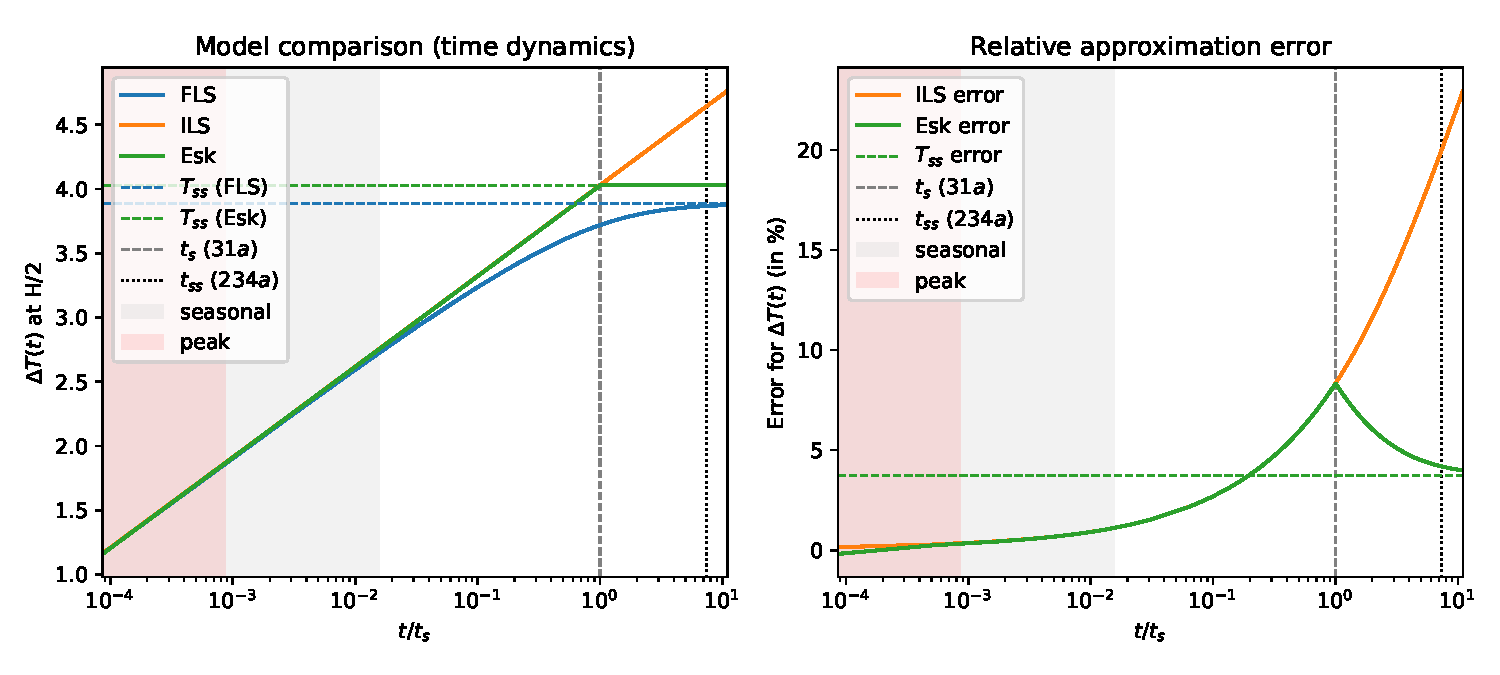
\includegraphics[width=.9\linewidth]{Figs/FLS_ILS_Esk_compare_ts.pdf}
    \caption{a) Temporal dynamics of the temperature variation along the borehole (shape of the "g-function") for the Finite Line Source (FLS), Infinite Line Source (ILS) and asymptotic (Esk) models, b) relative error for the temperature variation, as percentage of the $\Delta T_{FLS}$. The time duration of peak (red) and seasonal (grey) effects are highlighted.}
    \label{fig:T_dynamics}
\end{figure}

As mentioned above, the approximations of the FLS model are valid under certain assumptions, but may significantly speed-up the modelling time (even though the formulation in Eq.~\ref{eq:FLS_int} is already much faster than Eq.~\ref{eq:FLS}). To understand the ranges of validity and the error induced by the use of the approximations, we compare the different models for different time scales and distances to the borehole. All examples are shown for a borehole of 100m length, but the patterns are nearly identical for longer BHE's. In general, the temperature drop ($\Delta T$) along the borehole is smaller for larger $H$, hence leading to smaller absolute, but similar relative errors. 

Figure~\ref{fig:T_dynamics} shows a comparison between the models for different time scales at the borehole wall ($r = r_b$). We can see that for short time scales (red/grey), all models have a negligible error (up to $1\%$). 
Hence, any approximation may be used to model both peak and seasonal effects. At larger time scales, the ILS model starts to diverge from the FLS solution. 
This is expected, as the ILS never reaches a steady-state due to its infinite length. In this context, \citet{bandos_finite_2009} provide a formulation for a semi-infinite line source (SILS), which does reach a steady state. 

The Esk model is quasi-equivalent to the ILS for $t_{min} < t < t_s$, and reaches its steady-state for $t > t_s$. The figure shows that the upper asymptote overestimates the steady-state temperature by $3.7\%$, with the largest error occurring around $t = t_s$ ($\approx 8\%$). These percentages are valid for all borehole lengths. 
For typical boreholes of $H=100-200m$, the time scales with the maximum error (around $t_s$) correspond to the time scales of highest interest. 
As the absolute difference is relatively small, this may not have a large impact for modelling individual boreholes, and the asymptotic steady-state $\mathrm{g}_{Esk, qss}$ can be safely used. For modelling large borehole fields, however, the error accumulates, which can lead to significant differences in the estimated potential. For large-scale studies, the exact FLS solution should hence be used.

\begin{figure}[t]
    \centering
    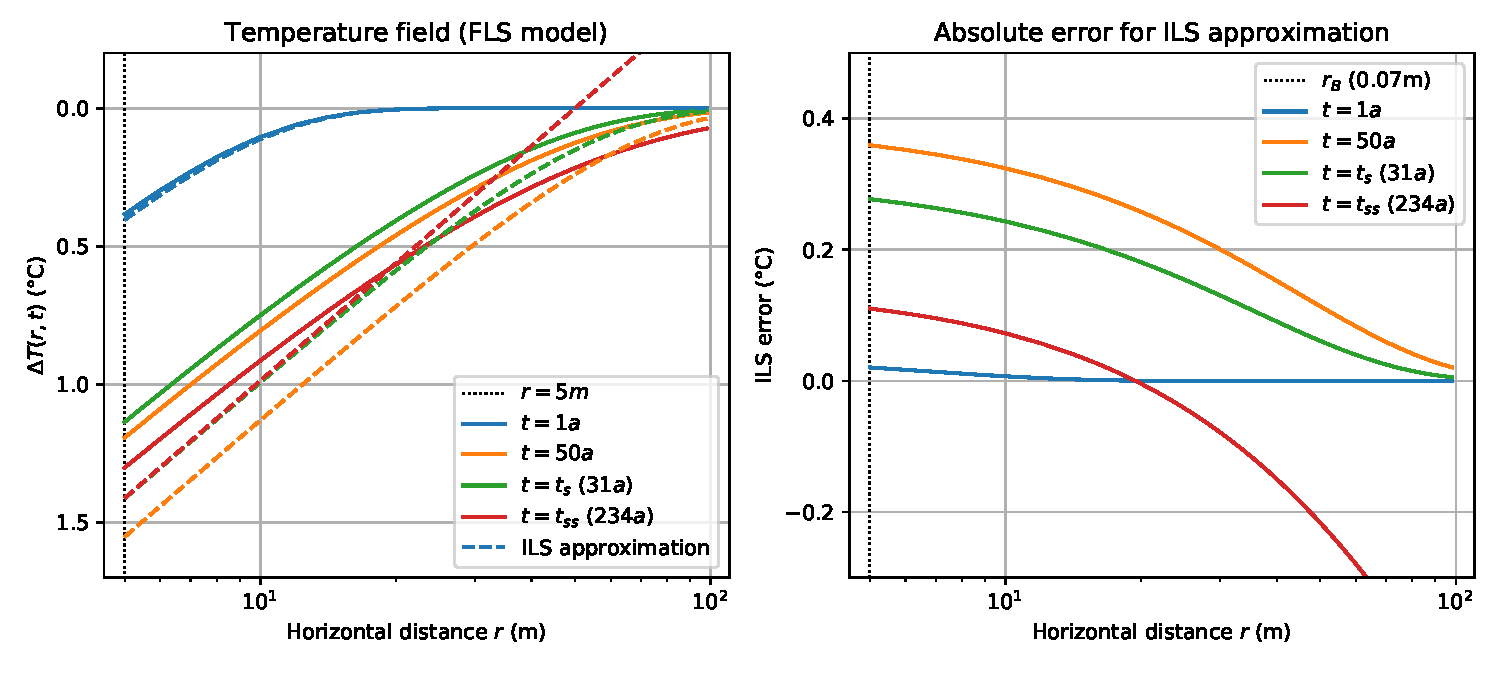
\includegraphics[width=.9\linewidth]{Figs/FLS_ILS_compare_r.pdf}
    \caption{a) Temperature field with distance to the BHE (length 100m) on logarithmic scale. The Infinite Line Source (with $\mathrm{g}_{Esk, qss}$ for $t = t_{ss}$) is shown for comparison (dashed lines). b) Absolute error (in $\circ$C) for the ILS model. The example shows a BHE of 100m length.}
    \label{fig:r_field}
\end{figure}

To assess the effect of adjacent boreholes, the temperature fields at large distances from the borehole ($5m < r < H$) are of interest. As seasonal and peak effects have a penetration depth that is lower than the minimum borehole distance of $5m$, only long-term effects are relevant. Figure~\ref{fig:r_field} shows the temperature drop in the ground for three long-term time intervals: the typical planning horizon ($t_{dim}$) for BHEs of 50 years, the quasi-steady-state $t_s$, where the temperature drop has reached around $95\%$ of its final value, and the actual steady state ($t_{ss}$). For comparison, also a short horizon of 1 year is shown.

While the temperature drop increases logarithmically for small distances, it trails off for distances that approach the borehole length $H$. In this range, Eq.~\ref{eq:apx} is no longer valid, so the transient asymptote cannot be used. This can be seen by the unrealistic steady-state solution, which represents the Esk steady-state asymptote (see Eq.~\ref{eq:Esk_qss}). It reaches a value of $0$ at $H/2$ and has negative values after, which is infeasible.

As Fig.~\ref{fig:T_dynamics} suggests, the error between the ILS and the FLS model increases with time, up to $0.1-0.3 ^\circ$C for the radii of interest. While this may  be negligible for a single neighbor, the error accumulates for borehole fields.  The exact FLS solution should hence be used for modelling large-scale geothermal potentials.


